\documentclass[tikz,border=2pt]{standalone}
% Preámbulo común de los diagramas TikZ (misma paleta y letra que las notas)
\usepackage[T1]{fontenc}\usepackage[utf8]{inputenc}
\usepackage{libertinus}\usepackage{libertinust1math}
\usepackage[defaultsans,scale=0.92]{lato}
\usepackage{amsmath,amssymb,bm}
\usepackage{tikz}\usetikzlibrary{calc,positioning,arrows.meta,shapes.geometric,decorations.pathreplacing,decorations.pathmorphing,fit,backgrounds}
\definecolor{snlazul}{HTML}{1E5AA8}\definecolor{snlnoche}{HTML}{14213D}\definecolor{snlvioleta}{HTML}{6C4AB6}
\definecolor{snlcoral}{HTML}{D1495B}\definecolor{snlambar}{HTML}{E09F3E}\definecolor{snlverde}{HTML}{2A9D8F}
\definecolor{snlteal}{HTML}{0F7173}\definecolor{snlgris}{HTML}{5C677D}\definecolor{snlfondo}{HTML}{F4F6FA}
\tikzset{>={Stealth[length=2.2mm]},
  bloque/.style={draw=#1,fill=#1!8,thick,rounded corners=2pt,minimum height=11mm,minimum width=20mm,align=center,font=\small},
  bloque/.default=snlazul,
  suma/.style={draw=snlnoche,thick,circle,inner sep=0pt,minimum size=5mm},
  flecha/.style={->,thick,draw=snlnoche},
  etq/.style={font=\small,text=snlnoche},
  nota/.style={font=\footnotesize\sffamily,text=snlgris,align=center}}

\begin{document}
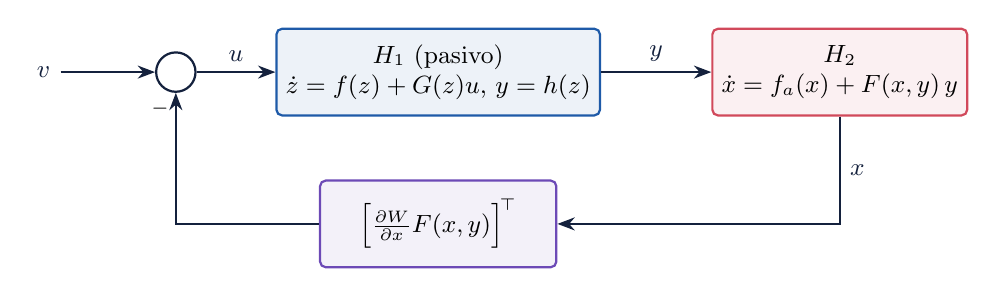
\begin{tikzpicture}
 \node[suma] (s) {};
 \node[bloque=snlazul,right=10mm of s,minimum width=30mm] (H1) {$H_1$ (pasivo)\\$\dot z=f(z)+G(z)u$, $y=h(z)$};
 \node[bloque=snlcoral,right=14mm of H1,minimum width=30mm] (H2) {$H_2$\\$\dot x=f_a(x)+F(x,y)\,y$};
 \node[bloque=snlvioleta,below=8mm of H1,minimum width=30mm] (K) {$\Bigl[\tfrac{\partial W}{\partial x}F(x,y)\Bigr]^{\!\top}$};
 \draw[flecha] ($(s.west)+(-12mm,0)$) node[left,etq]{$v$} -- (s);
 \draw[flecha] (s) -- node[above,etq]{$u$} (H1);
 \draw[flecha] (H1) -- node[above,etq]{$y$} (H2);
 \draw[flecha] (H2.south) |- (K.east) node[pos=0.25,right,etq]{$x$};
 \draw[flecha] (K.west) -| (s.south);
 \node[font=\scriptsize] at ($(s.south)+(-2mm,-2mm)$) {$-$};
\end{tikzpicture}
\end{document}
